\documentclass[12pt]{article}

\usepackage[utf8]{inputenc}
\usepackage{geometry}
\geometry{a4paper, margin=1in}
\usepackage{titlesec}
\usepackage{listings}
\usepackage{graphicx}
\title{\Large Final Project Report: EECE2140 COMPUTING FUNDAMENTALS FOR ENGINEERS}
\author{
    \normalsize Enocder/Decoder project\\
    \normalsize Student Names: Noah Yue and Isaac Rounds \\
    \normalsize Northeastern University \\
    \normalsize College of Engineering \\
    \normalsize Department of Electrical and Computer Engineering \\
    \normalsize Course Title: EECE 2140: COMPUTING FUNDAMENTALS FOR ENGINEERS \\
    \normalsize Instructor: Fatema Nafa \\
    \normalsize Spring Semester 2024
}
\date{\normalsize\today}

\begin{document}

\maketitle
\newpage


\section{Abstract}
The objective of our project was to create a program capable of reading data from a file, encoding or decoding it, and then writing the finished product to a new file. The program was written in Python and uses a basic command prompt user interface. The library cryptodome was used for creating cipher objects and the code is primarily structured using classes. 

The program created successfully reads .txt and .pdf files (for reading .pdf files the library pypdf was used), encodes or decodes, and then writes to a .txt file

this program uses three ciphers: Shift, DES (Data Encryption Standard), and AES (Advanced Encryption Standard). 

DES and AES encode and decode their data in bits - because of this this project is also capable of converting strings to bits and vice versa.




\section{Objective and Introduction}

This program was designed to read data from .pdf and .txt files, encode or decode that data (in AES, DES, or using shift encryption) and then write the results to a .txt file.
Data encryption is an extraordinarily important part of the modern internet. Gaining an understanding of how data encryption works is very important to us, as future engineers who will be responsible for designing projects that are secure. To get an understanding of encryption from the ground up we designed an extraordinarily simple cipher first, the shift cipher. Then we made the DES cipher, which is now obsolete. Finally we designed the AES cipher, which is still in use today.

\section{Theory and Experimental Methods}

Our code was almost always in functions or classes. We did this for two reasons- it improved readability and having our code easily segmented allowed both of us to work on separate files simultaneously. Keeping our code very segmented also allowed us to easily deduce where a bug was originating from and fix the error. The naming of our functions and classes was important because of how frequently they were used. All cipher classes were named [cipher type]Cipher, and of those cipher classes all have a method called encrypt and decrypt, which encrypt and decrypt data sent to them when called.



We made cyphers using classes
and other junk with functions

\section{Results}
Code input and output:
\begin{center}
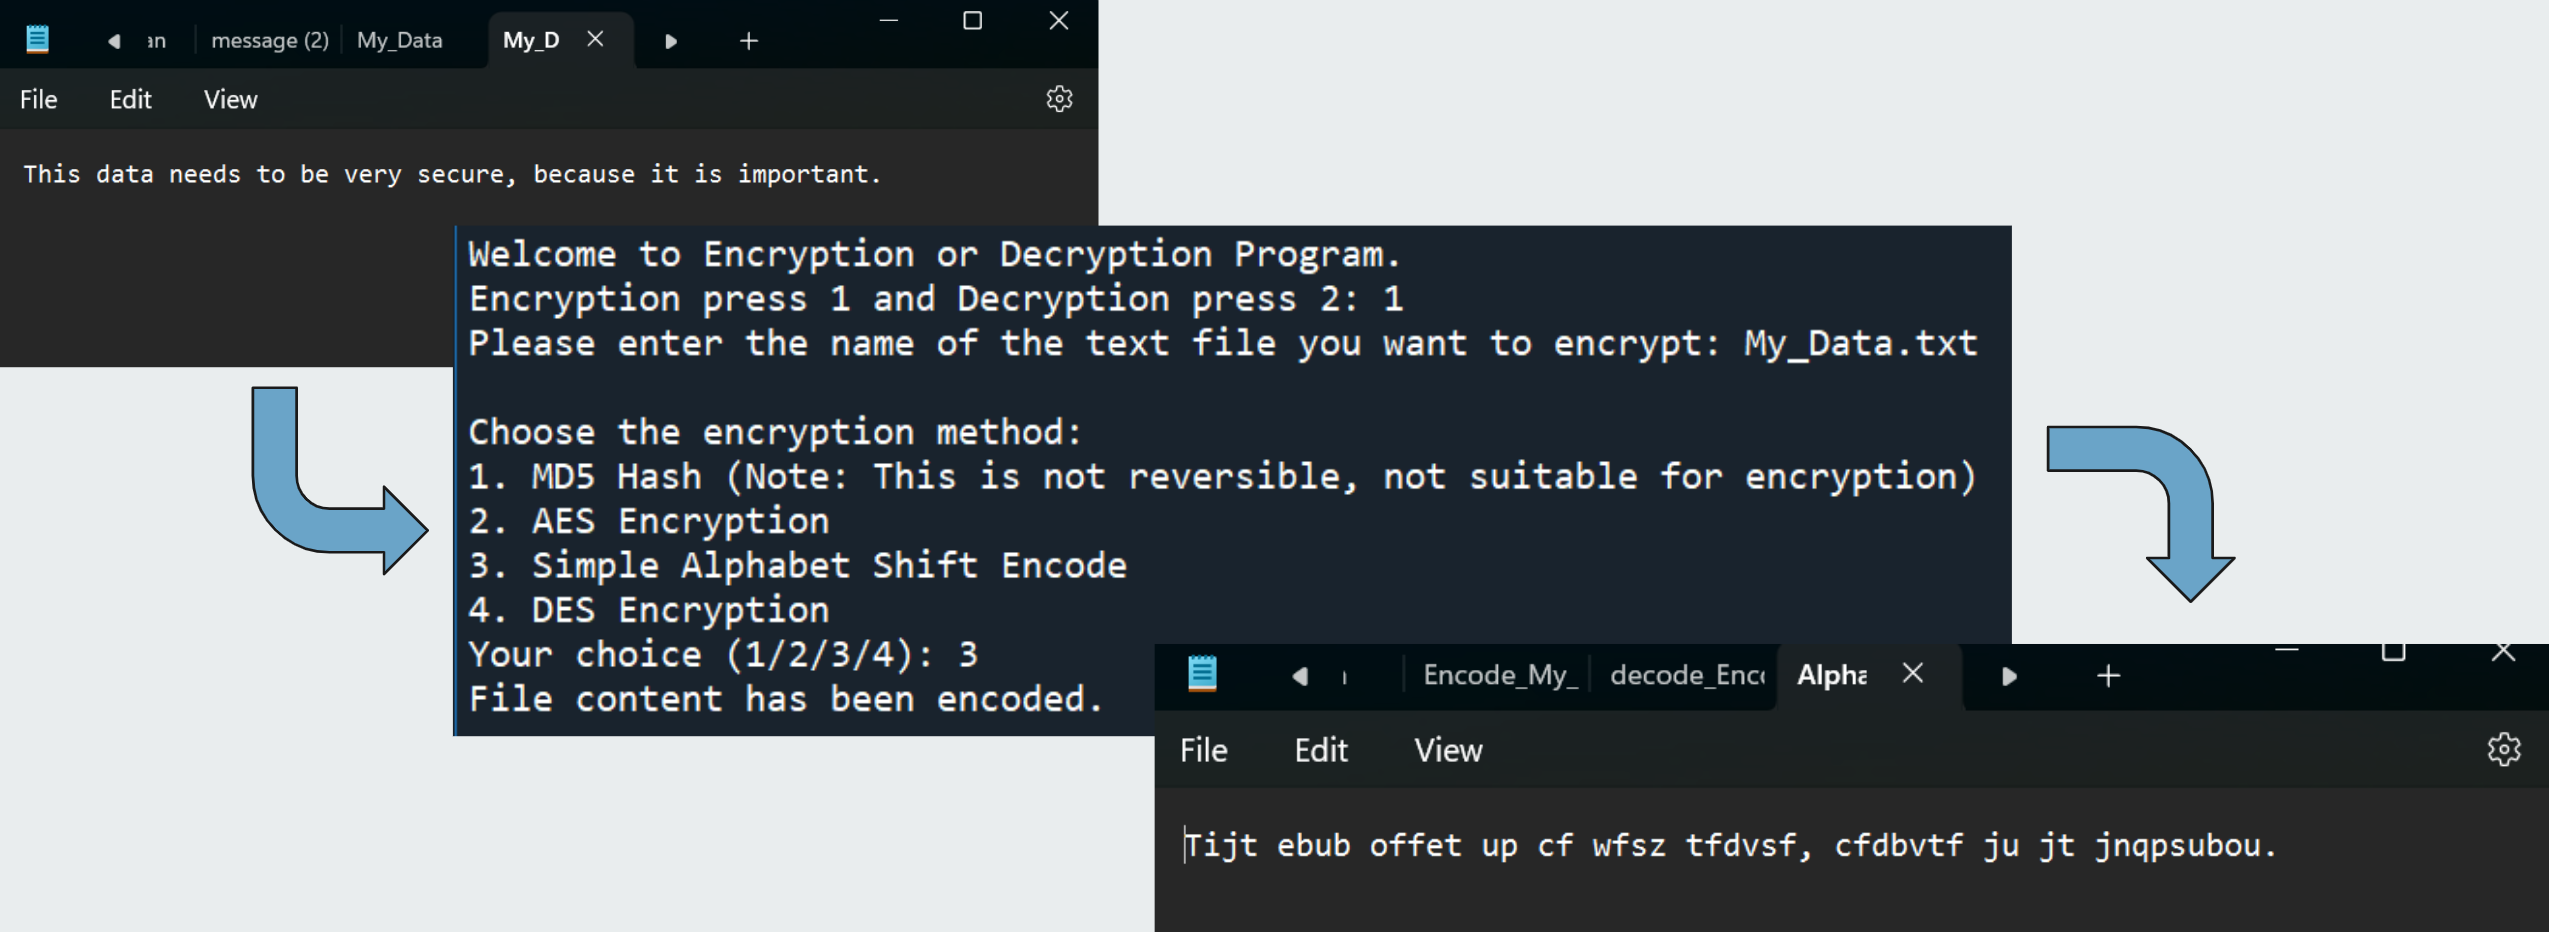
\includegraphics[width=1\linewidth]{image.png}
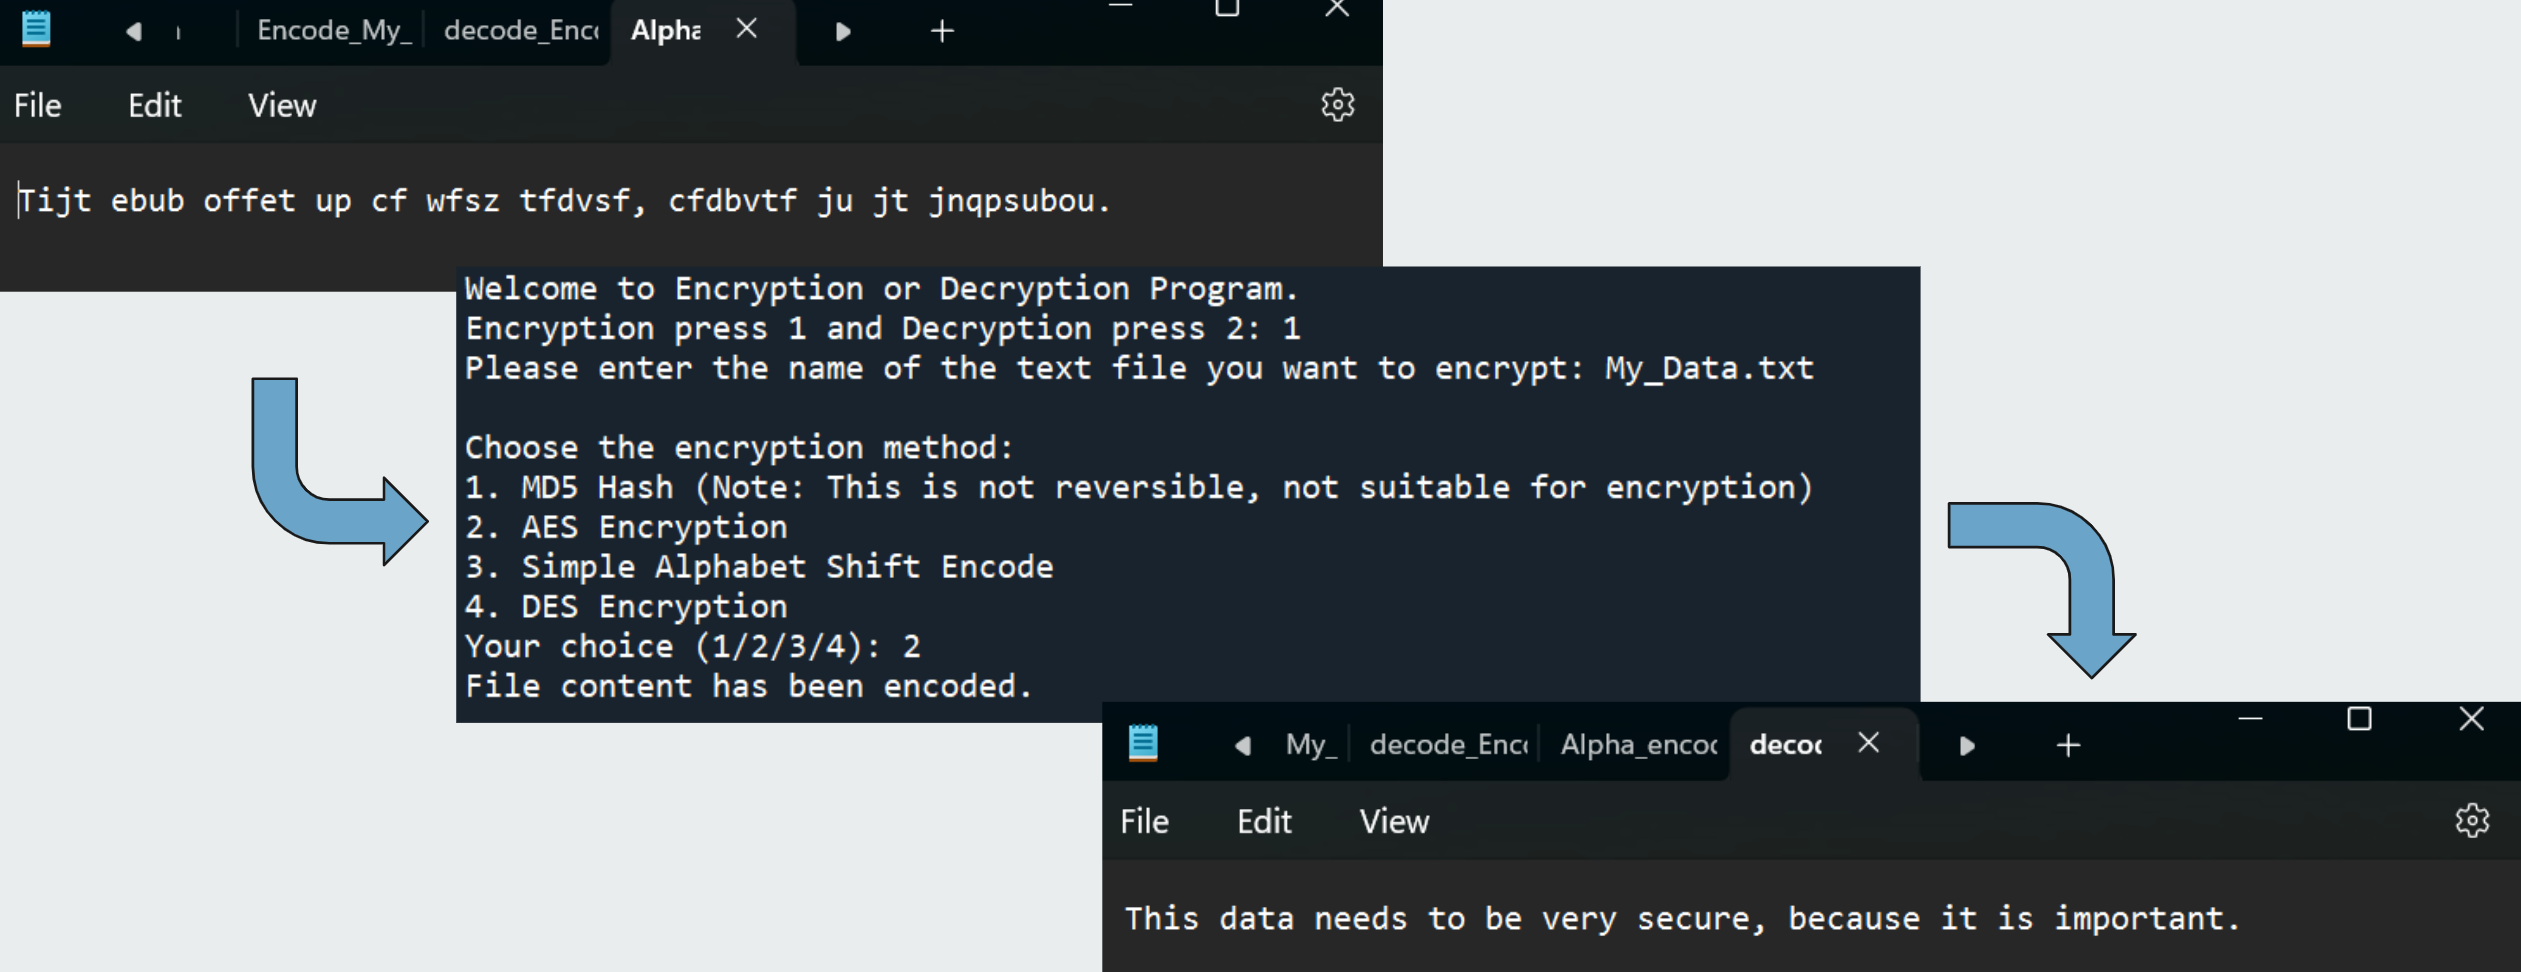
\includegraphics[width=1\linewidth]{1.png}
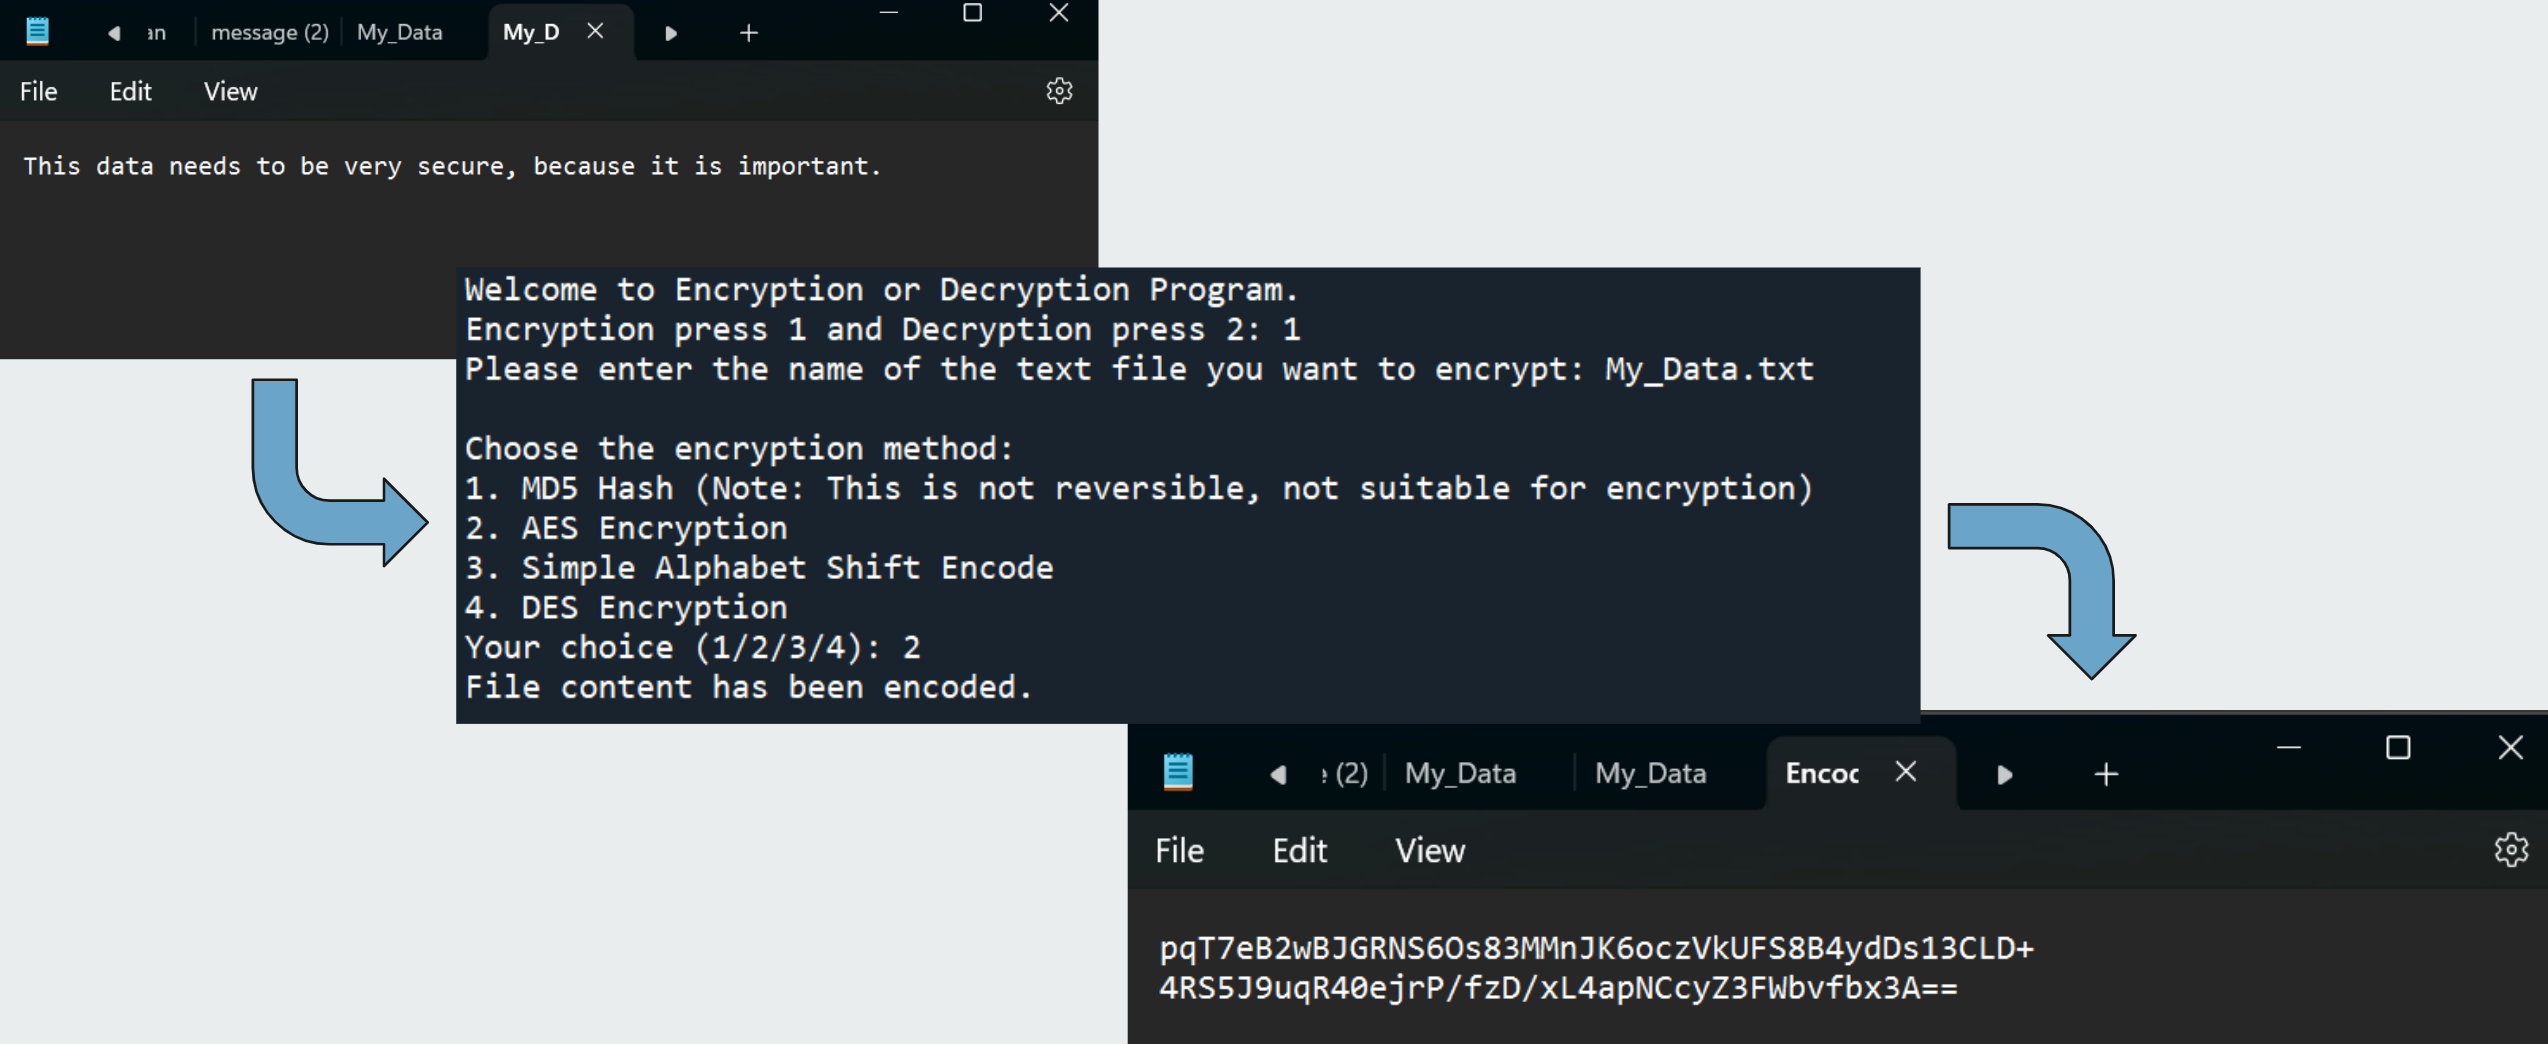
\includegraphics[width=1\linewidth]{2.png}
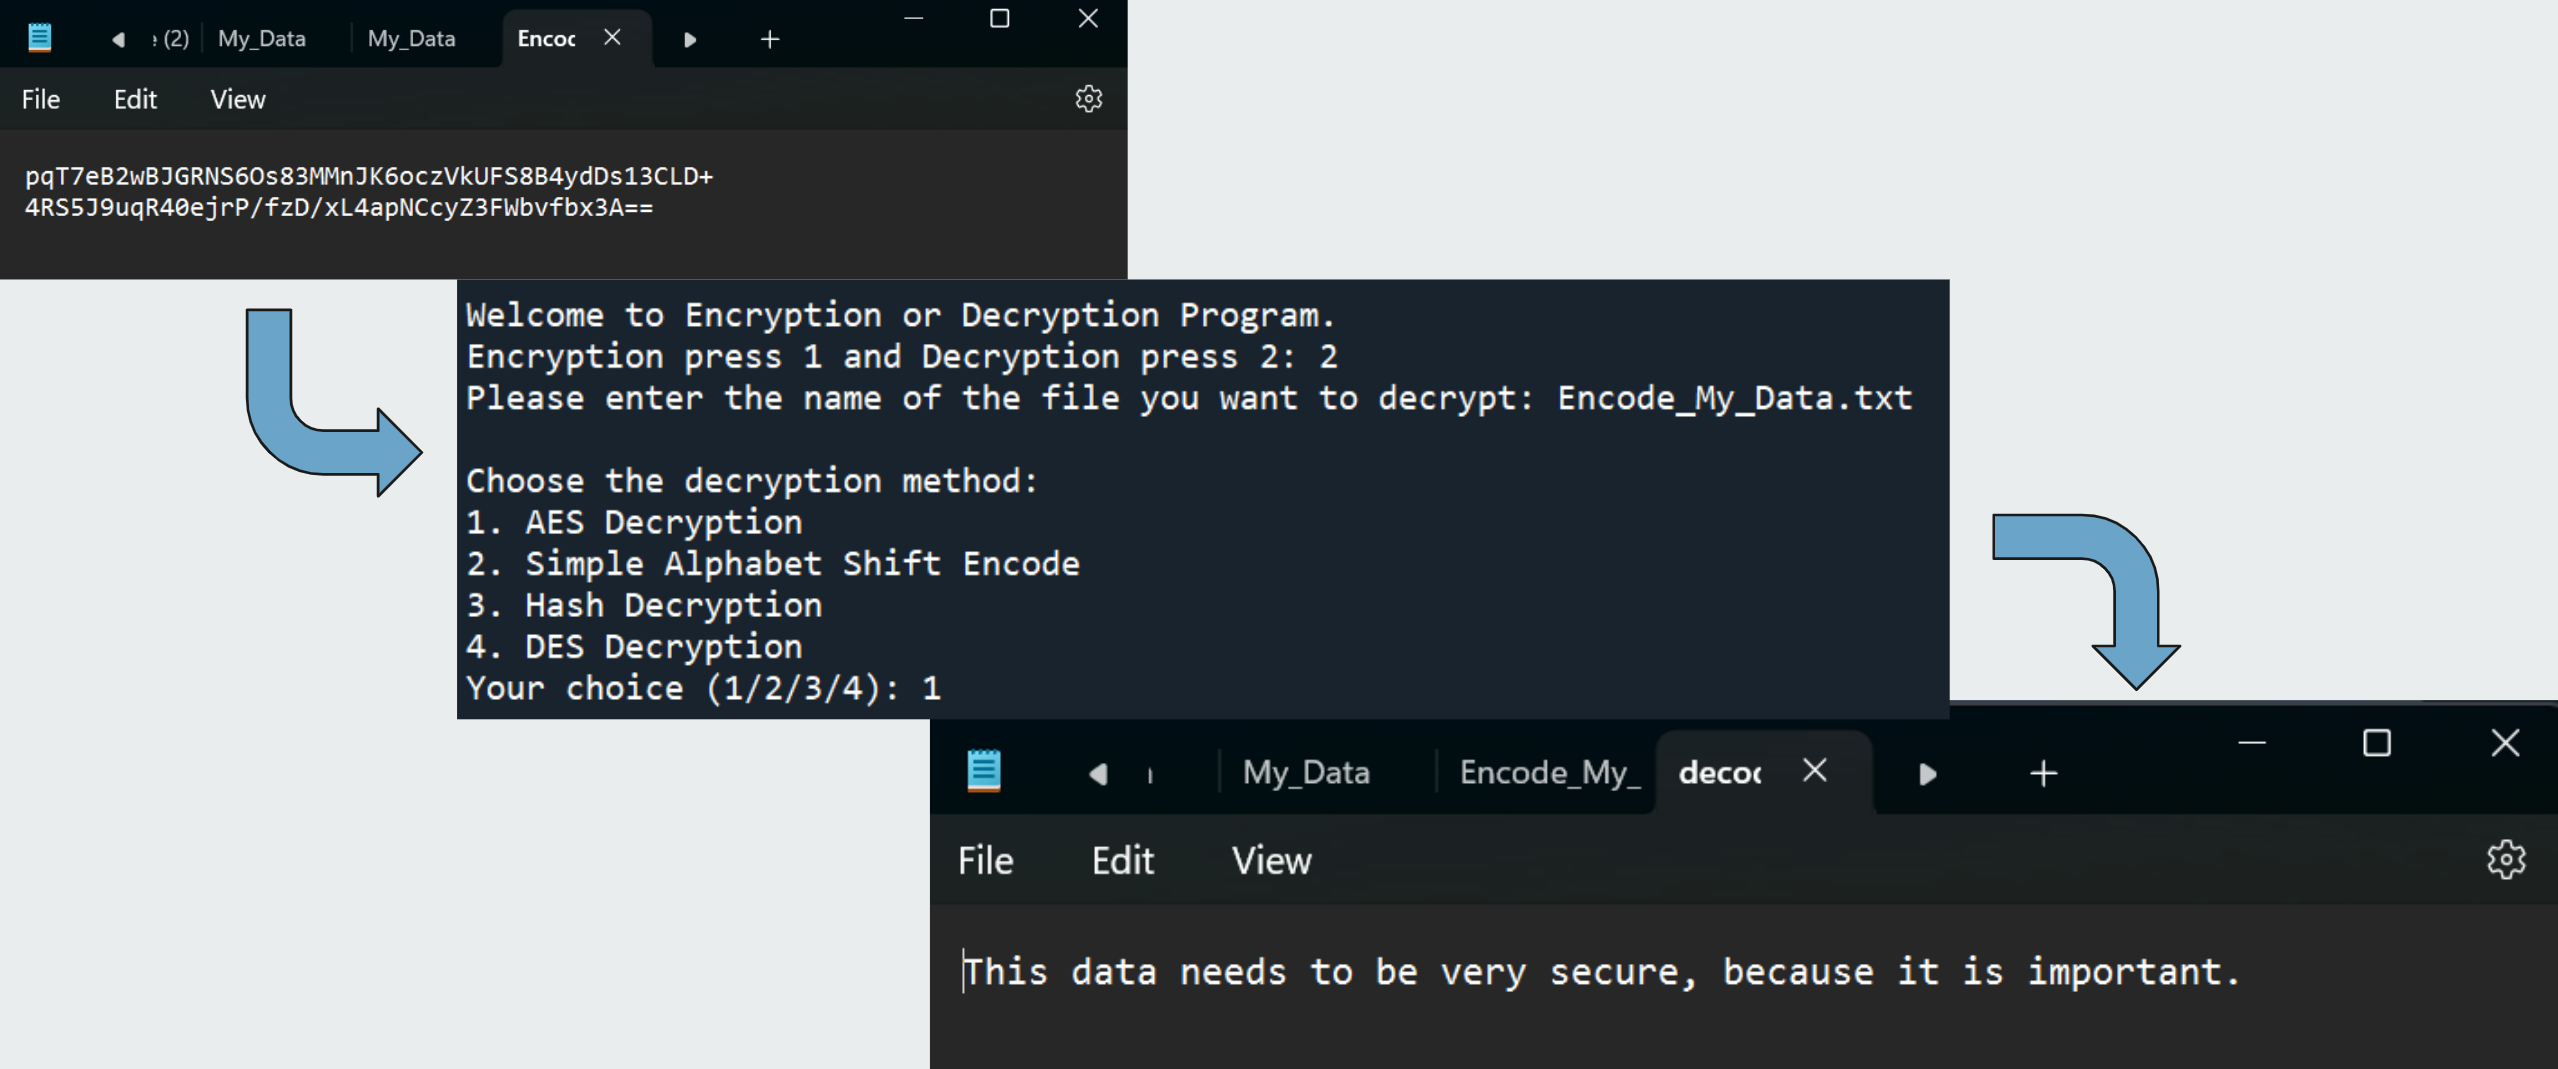
\includegraphics[width=1\linewidth]{3.png}
\end{center}

\section{Conclusions}
The program was successful. It is able to encode and decode data as well as reading and writing to .txt files. We learned more about how ciphers function, including ciphers used in the modern day. We now understand more about how ciphers take binary data and scramble/unscramble the bits.
\section{Limitations and Future Work}
the program is unable to write to .pdf files. This is because the pypdf library does not support writing to .pdf files. The pypdf library is also not 100 percent reliable when reading from pdfs. The program also does not save new lines in the encrypted data, so when data is run through the program it will not have the new line's the original did.
A future feature that would improve the usefulness of the program is a way for the program to attempt to figure out what cipher the encoded data needs to be decoded.
\section{References}
\begin{itemize}
    \item https://blog.csdn.net/chouzhou9701/article/details/12201996
    \item https://sectigostore.com/blog/what-is-des-encryption-a-look-at-the-des-algorithm/
    \item https://pypi.org/project/pycryptodome/
    \item https://pypi.org/project/pypdf/
    \item https://docs.python.org/3/library/hashlib.html
    \item https://docs.python.org/3/library/base64.html
\end{itemize}
\end{document}